

\tikzset{every picture/.style={line width=0.75pt}} %set default line width to 0.75pt        

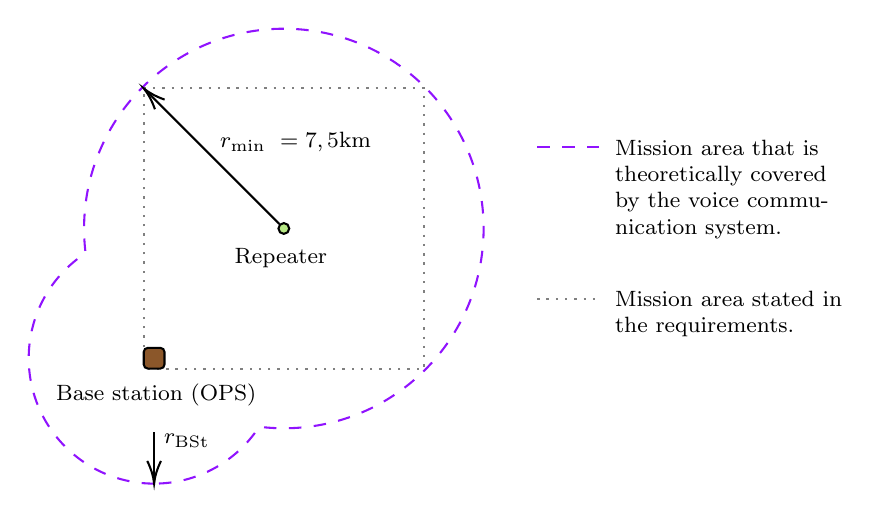
\begin{tikzpicture}[x=0.75pt,y=0.75pt,yscale=-1,xscale=1]
%uncomment if require: \path (0,409); %set diagram left start at 0, and has height of 409

%Shape: Rectangle [id:dp12443341375434458] 
\draw  [color={rgb, 255:red, 128; green, 128; blue, 128 }  ,draw opacity=1 ][dash pattern={on 0.84pt off 2.51pt}] (105.42,168.75) -- (240.42,168.75) -- (240.42,303.75) -- (105.42,303.75) -- cycle ;
%Shape: Path Data [id:dp8368288281183056] 
\draw  [color={rgb, 255:red, 144; green, 19; blue, 254 }  ,draw opacity=1 ][dash pattern={on 4.5pt off 4.5pt}] (110.42,359.17) .. controls (77.05,359.17) and (50,332.12) .. (50,298.75) .. controls (50,277.57) and (60.9,258.93) .. (77.4,248.14) .. controls (76.92,244.24) and (76.67,240.28) .. (76.67,236.25) .. controls (76.67,183.09) and (119.77,140) .. (172.92,140) .. controls (226.08,140) and (269.17,183.09) .. (269.17,236.25) .. controls (269.17,289.41) and (226.08,332.5) .. (172.92,332.5) .. controls (168.9,332.5) and (164.93,332.25) .. (161.04,331.77) .. controls (150.25,348.27) and (131.61,359.17) .. (110.42,359.17) -- cycle ;
%Rounded Rect [id:dp41901798669291956] 
\draw  [fill={rgb, 255:red, 139; green, 87; blue, 42 }  ,fill opacity=1 ] (105.42,295.75) .. controls (105.42,294.65) and (106.32,293.75) .. (107.42,293.75) -- (113.42,293.75) .. controls (114.53,293.75) and (115.42,294.65) .. (115.42,295.75) -- (115.42,301.75) .. controls (115.42,302.85) and (114.53,303.75) .. (113.42,303.75) -- (107.42,303.75) .. controls (106.32,303.75) and (105.42,302.85) .. (105.42,301.75) -- cycle ;
%Straight Lines [id:da8105217749265208] 
\draw    (110.42,357.17) -- (110.42,334.17) ;
\draw [shift={(110.42,359.17)}, rotate = 270] [color={rgb, 255:red, 0; green, 0; blue, 0 }  ][line width=0.75]    (10.93,-3.29) .. controls (6.95,-1.4) and (3.31,-0.3) .. (0,0) .. controls (3.31,0.3) and (6.95,1.4) .. (10.93,3.29)   ;
%Straight Lines [id:da3146532721436186] 
\draw    (106.84,170.16) -- (170.74,234.06) ;
\draw [shift={(105.42,168.75)}, rotate = 45] [color={rgb, 255:red, 0; green, 0; blue, 0 }  ][line width=0.75]    (10.93,-3.29) .. controls (6.95,-1.4) and (3.31,-0.3) .. (0,0) .. controls (3.31,0.3) and (6.95,1.4) .. (10.93,3.29)   ;
%Shape: Circle [id:dp5997567206989125] 
\draw  [fill={rgb, 255:red, 184; green, 233; blue, 134 }  ,fill opacity=1 ] (170.32,236.25) .. controls (170.32,234.81) and (171.49,233.65) .. (172.92,233.65) .. controls (174.36,233.65) and (175.52,234.81) .. (175.52,236.25) .. controls (175.52,237.69) and (174.36,238.85) .. (172.92,238.85) .. controls (171.49,238.85) and (170.32,237.69) .. (170.32,236.25) -- cycle ;
%Straight Lines [id:da1970463822196904] 
\draw [color={rgb, 255:red, 144; green, 19; blue, 254 }  ,draw opacity=1 ] [dash pattern={on 4.5pt off 4.5pt}]  (295,197) -- (325,197) ;

%Straight Lines [id:da2827334971957638] 
\draw [color={rgb, 255:red, 128; green, 128; blue, 128 }  ,draw opacity=1 ] [dash pattern={on 0.84pt off 2.51pt}]  (295,270) -- (325,270) ;


% Text Node
\draw (331,192) node [anchor=north west][inner sep=0.75pt]  [font=\footnotesize] [align=left] {Mission area that is \\theoretically covered\\by the voice commu-\\nication system. };
% Text Node
\draw (61.74,309.44) node [anchor=north west][inner sep=0.75pt]  [font=\footnotesize] [align=left] {Base station (OPS)};
% Text Node
\draw (147.74,244.44) node [anchor=north west][inner sep=0.75pt]  [font=\footnotesize] [align=left] {Repeater};
% Text Node
\draw (113.74,333.84) node [anchor=north west][inner sep=0.75pt]  [font=\footnotesize]  {$r_{\mathrm{BSt}}$};
% Text Node
\draw (140.74,188.46) node [anchor=north west][inner sep=0.75pt]  [font=\footnotesize]  {$r_{\mathrm{min}} \ =7,5\mathrm{km}$};
% Text Node
\draw (331,265) node [anchor=north west][inner sep=0.75pt]  [font=\footnotesize] [align=left] {Mission area stated in\\the requirements.};


\end{tikzpicture}
